\section{Project guidelines}
\subsection{Deployment plan}
\subsubsection{Scheduling and Timeframes}
   
\begin{center}
    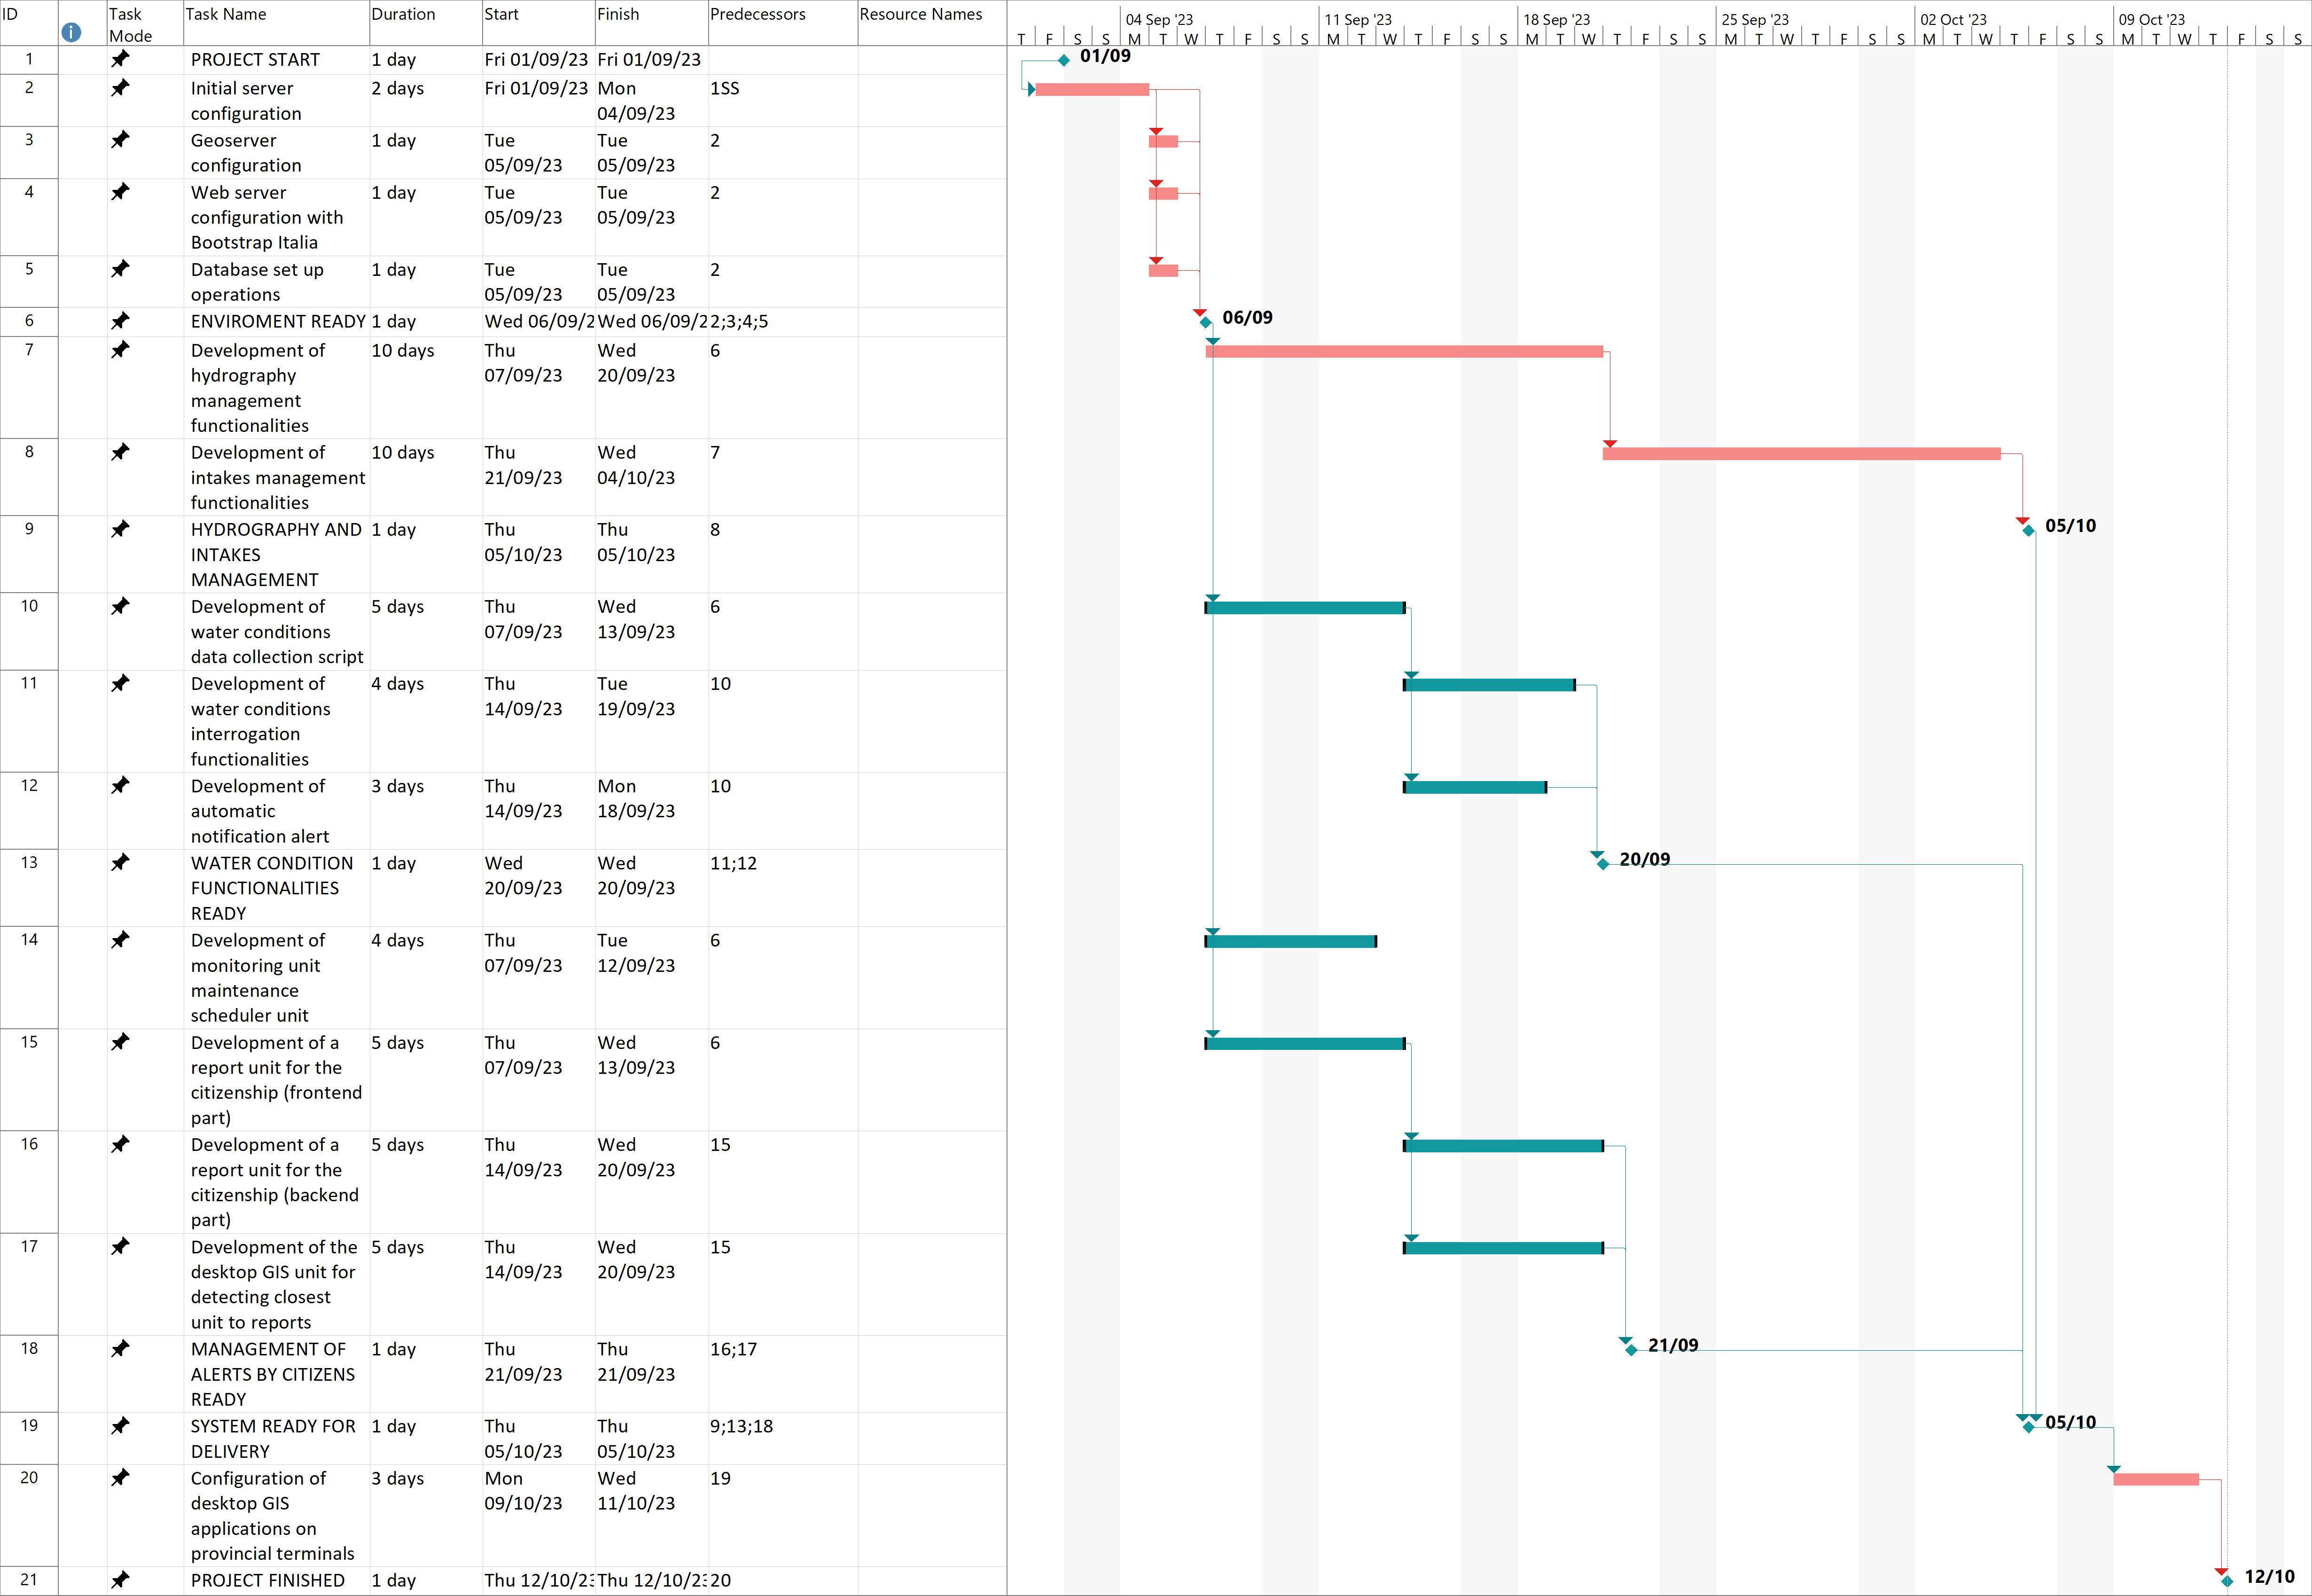
\includegraphics[width=\textwidth]{img/gantt.png}
\end{center}

\subsubsection{Description}
In the Gantt chart are shown all the activities necessary to reach the final goal; the working hypotesis is to start the project by the 1st of September 2023 with the sever configuration procedures and then finish up everything (if no delays happens) by the 12th of October: the whole execution then should take around one month and a half.
This hypotesis does not take care of the number of working resources (software engineers or programmers) available for the execution, that can led to a more constrained execution due to many parallelized activities. \\
Activities coloured in pink represents the \textit{critical path}, that are the ones in which a delay can led to a delay of the whole project.

\subsection{Deliverables}
From the Gantt chart is visible that three main milestone are present in the timeline of the project: these coincides with three different \textit{deliverables}, that are three tangible and atomically usable parts of the system.\\
In particular:
\begin{itemize}
    \item \textbf{05/10}: this deliverable coincides with the delivery of the hydrography and intakes management functionalities. Theoretically, from this date the provincial emplyees can start to use and to test this subpart of the system;
    \item \textbf{20/09}: this deliverable coincides with the delivery of the automatic data reading subsystem from the web gateways and the email alert system. Theoretically, from this date the provincial emplyees can start to use and to test this subpart of the system;
    \item \textbf{21/09}: this deliverable coincides with the delivery of the reporting subsystem for the citizenship and its backend and desktop management functionalities. Theoretically, from this date the provincial emplyees can start to use and to test this subpart of the system.
\end{itemize}